\documentclass{article}

%\documentclass[10pt,twocolumn]{article}

% if you need to pass options to natbib, use, e.g.:
% \PassOptionsToPackage{numbers, compress}{natbib}
% before loading nips_2017
%
% to avoid loading the natbib package, add option nonatbib:
\usepackage[nonatbib]{nips_2017}




% to compile a camera-ready version, add the [final] option, e.g.:
\usepackage{algorithm}
\usepackage[noend]{algpseudocode}
\usepackage{times}
\usepackage{float}
\usepackage {tikz}
\usepackage{amsmath}
\usepackage{amsfonts}
%\usepackage{graphicx}
%\usepackage[pdftex]{graphicx}
\pagestyle{plain} 
\newcommand{\RNum}[1]{\uppercase\expandafter{\romannumeral #1\relax}}

\setlength\parindent{24pt}
\DeclareMathOperator{\E}{\mathbb{E}}
\begin{document}

\title{Generative Modeling With Vine Models}

\maketitle
\section{Formulation}
The goal is to optimize the construction of the vine copula model in order to minimize the Wasserstein distance between the true underlying distribution and the distribution of model. 
The construction of the first tree can be seen as a sequential decision making process: in each step we select a variable and link it with a variable in the existing tree. Therefore it is natural to model the process in the syntax of Reinforcement Learning. 

Let $\mathbb{P}_r$ be the true underlying distribution and $\mathbb{P}_g$ be the distribution of the vine copula model used to generated synthetic data.
The Wasserstein-1 distance is defined as:
\[
W(\mathbb{P}_r,\mathbb{P}_g)=\sup_{||f||_L\leq1}\mathbb{E}_{x\sim\mathbb{P}_r}[f(x)]-\mathbb{E}_{x\sim\mathbb{P}_g}[f(x)]
\]
where the supremum is over all the 1-Lipschitz functions.
There are two choices that can be made:
\begin{enumerate}
    \item The choices of bi-variate copula functions (Is that possible to locally search for the best bi-variate copula function subject to some constraints.)
    \item The sequence of variables to join when construct the vine
\end{enumerate}



For a fix generator, the discriminator solves the following optimization problem:
\[

\]
\section{Related Work}













\section{Sampling}

\begin{tikzpicture}[auto, node distance=2cm,main node/.style={draw}]
\node[main node] (1) {1};
\node[main node] (2) [right of=1] {2};
  \node[main node] (3) [right of=2] {3};
  \node[main node] (4) [right of=3] {4};

  \path[every node/.style={font=\sffamily\Large\bfseries}]
    (1) edge node {$C_{1,2}$} (2)
    (2) edge node {$C_{2,3}$} (3)
    (3) edge node {$C_{3,4}$} (4)
\end{tikzpicture}

\begin{tikzpicture}[auto, node distance=2.5cm,main node/.style={draw}]

  \node[main node] (1) {1,2};
  \node[main node] (2) [right of=1] {2,3};
  \node[main node] (3) [right of=2] {3,4};

  \path[every node/.style={font=\sffamily\Large\bfseries}]
    (1) edge node {$C_{1,3|2}$} (2)
    (2) edge node {$C_{2,4|3}$} (3)
\end{tikzpicture}

\begin{tikzpicture}[auto, node distance=3cm,
                    main node/.style={draw}]
  \node[main node] (1) {$2,3|1$};
  \node[main node] (2) [right of=1] {$2,4|3$};

  \path[every node/.style={font=\sffamily\Large\bfseries}]
    (1) edge node {$C_{1,4|2,3}$} (2)
\end{tikzpicture}


	The sampling procedure requires a complete vine model of n nodes $X_1,X_2,...,X_n$, and their corresponding marginal distribution $F_1,F_2,...,F_n$.
Considering the case where we have a D-Vine model with 4 nodes. We start by sampling uni-variate distribution $u_1,u_2,u_3,u_4$ from Uniform Distribution over [0,1]. We randomly pick a node to start with, say $X_2$.

Then the first variable $x_2 \sim X_2$ can be sampled as:
\begin{align}
x_2 = F_2^{-1}(u_2)
\end{align}
After we have $x_2$, we randomly pick a node connected to $X_2$. Suppose we pick $X_3$, recall that the conditional density $f_{3|2}$ can be written as:
\begin{align}
f_{3|2}(x_3|x_2)&=f_3(x_3)c_{2,3}(F_2(x_2),F_3(x_3)) \\
&=f_3(x_3)c_{2,3}(u_2,u_3) \\
&=f_3(x_3)c_{3|2}(u_3)
\end{align}
Thus, $x_3 \sim X_3|X_2$ can be sampled by:
\begin{align}
x_3 = F_3^{-1}(C_{3|2}^{-1}(u_3))
\end{align}
where $C_{3|2}$ can be obtained from $C_{2,3}$ in $T_1$ by plugging in sampled values of $u_2$. 

Similarly, we pick a node that shares an edge with $X_3$, say $X_4$. Then $x_4 \sim X_4|X_2,X_3$ can be sampled as:
\begin{align}
x_4= F_4^{-1}\circ C_{4|3}^{-1}\circ C_{4|23}^{-1}(u_4)
\end{align}
Finally $x1 \sim X_1|X_2,X_3,X_4$ can be sampled as:
\begin{align}
x_1= F_1^{-1}\circ C_{1|4}^{-1}\circ C_{1|34}^{-1}\circ C_{1|234}^{-1}(u_1)
\end{align}

For a more general vine graph, we can use a modified Breadth First Search to traverse the tree and keep track of nodes that have already been sampled. The general procedure is described below:
\begin{algorithm}
\caption{Generative Modeling with Vine Models}\label{euclid}
\begin{algorithmic}[1]
\Procedure{Sampling}{}
\State $\textit{explore} \gets \text{Queue()}$
\State $\textit{visited} \gets \text{list()}$
\State $start \gets \text{randomly chosen start node}$
\State \textit{explore}.\text{enqueue(start)}
\While {\text{explore not empty}}
\State $cur \gets \textit{explore.}\text{dequeue()}$
\State $i \gets \text{len(visited)}$
\State $x_{cur} = F_{cur}^{-1}\circ C_{cur|visited[i-1]}^{-1}...\circ C_{cur|visited[1,..,i-1]}^{-1}(u_{cur})$
 \For{\text{s $\in$ neighbor(cur)}}
        \If{s $\in$ visited}
                \State Continue
        \Else
        		\State \textit{explore}.\text{enqueue(s)}
        \EndIf
\State \textit{visited}.\text{left\_append(\textit{cur})}
\EndFor
\EndWhile
\EndProcedure
\end{algorithmic}
\end{algorithm}

\section{Experiment}
\begin{figure}
    \centering
    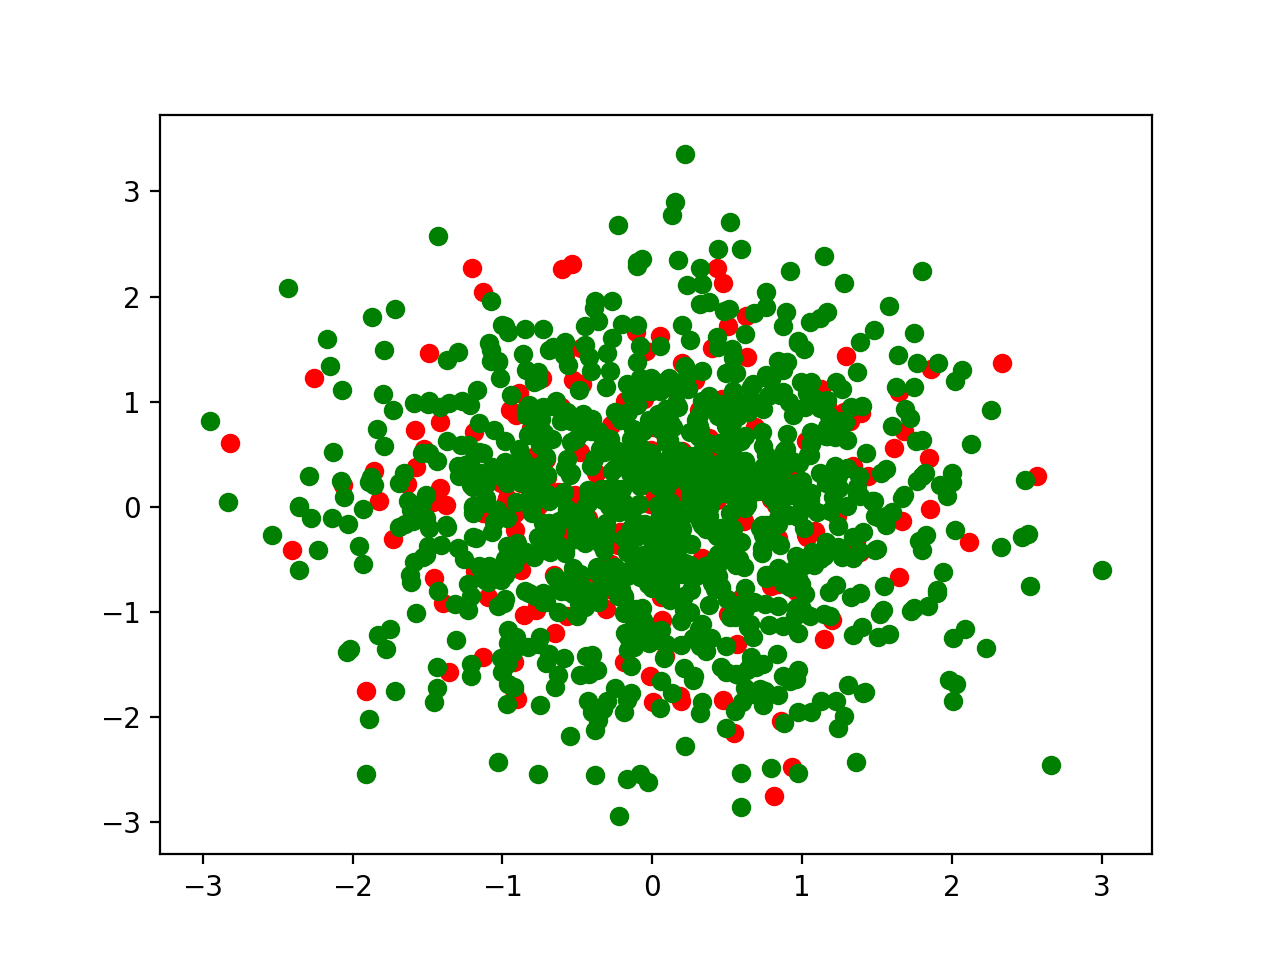
\includegraphics[scale=0.6]{ind_gaussian.png}
    \caption{Independent Gaussian}
    \label{fig:my_label}
\end{figure}

\begin{figure}
    \centering
    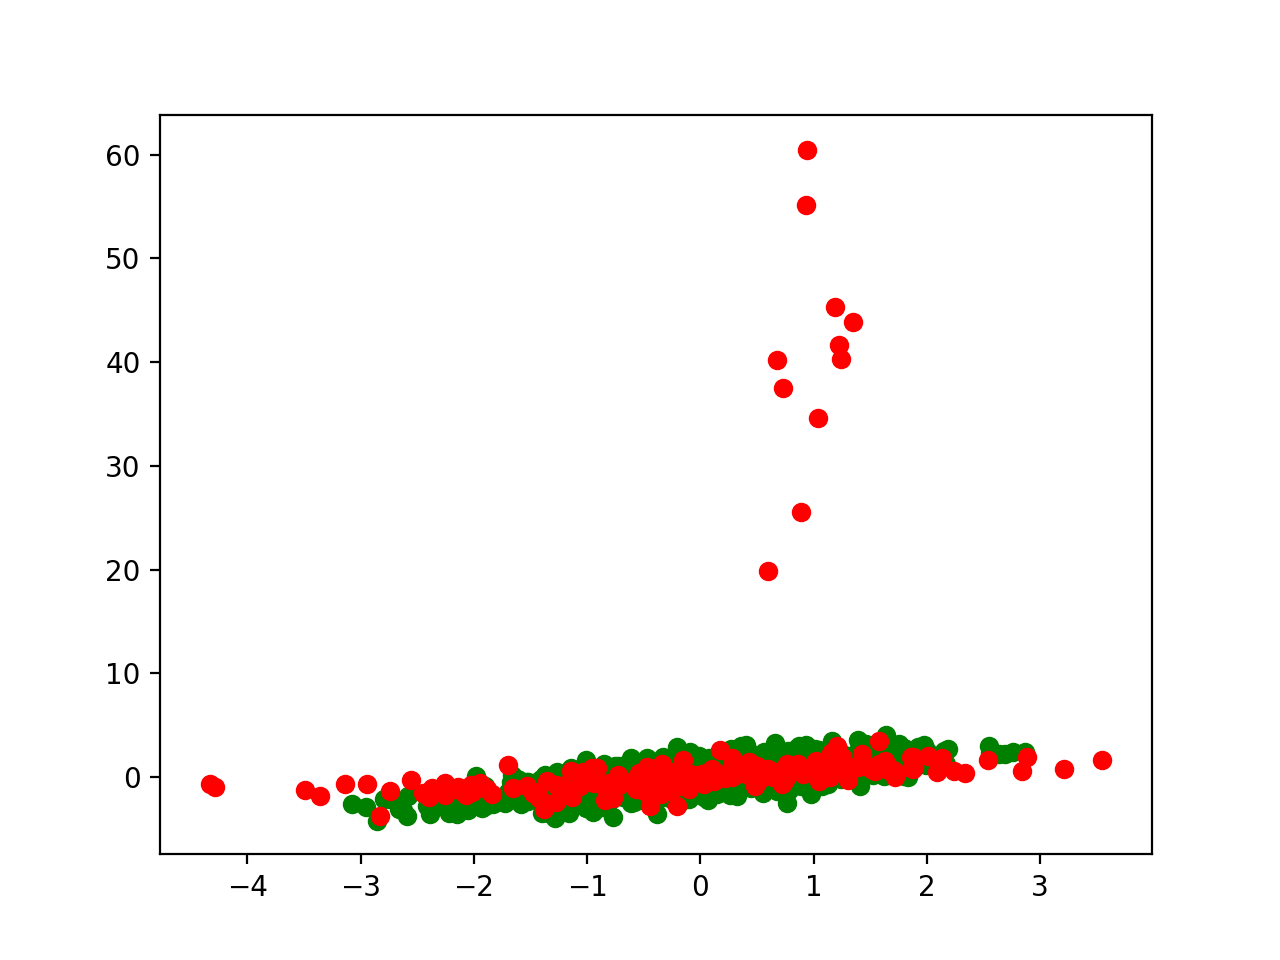
\includegraphics[scale=0.6]{correlated_gaussian.png}
    \caption{Correlated Gaussian}
    \label{fig:my_label}
\end{figure}









\end{document}